\section{Appendix}


\TheoremInvActRobbermonotonicity*
\begin{proof}
    First of all, a speed bound only puts restrictions on the robber and not the cops; therefore, $\rmiacopwidth{s}(G) \leq \rmiacopwidth{\infty}(G)$. To prove the other direction, assume we have $\rmiacopwidth{s}(G)=k$ and let $f$ be a corresponding search strategy. For contradiction, assume that there is a play with a robber $(R_t)_{t\in\N}$ of infinite speed that does not get caught in it. Lets call $Z_t = \bigcup_{t'\leq t}S_{t'}$ the cleared zone at the start of round $t$. Let $t'$ be the smallest index that satisfies $R_{t'} \in Z_{t'}$ and assume it exists. Then $R_{t'} \in Z_{t'-1}$, because the robber does not get caught and $R_{t'-1} \notin Z_{t'-1}$, so there is path in $G\setminus \{S_{t'} \cap S_{t'-1}\}$ from $R_{t'-1}$ to $R_{t'}$ containing an edge $vw$ with $v\notin Z_{t'-1}$ and $w\in Z_{t'-1}$.
    So, at either round $t'-1$ or $t'$, the vertex $w$ is not occupied by a cop but has been in an earlier round; we call this round $\tilde{t}$. $v$ is not occupied for the first $t'-1$ rounds, so a robber could, regardless of its speed, wait at $v$ until round $\tilde{t}$ and then move to $w$ without getting caught, contradicting that the search strategy $f$ is robber\-/monotone for finite speeds. So no such $t'$ can exist and as $(R_t)_{t\in\N}$ does not get caught, he must remain outside $Z_t$, so $Z_t \neq V$ for all $t$. However, a speed\-/bound robber could then just stay at a vertex $v\in V\setminus \bigcup_{t}Z_{t}$ that is never visited by the cops and remains uncaught. This contradicts that $f$ is a winning cop strategy, and we get $\rmiacopwidth{\infty}(G)=k$ because our strategy is still robber\-/monotone.
\end{proof}

\TheoremInvLazyCopmonotonicity*
\begin{proof}
    $\cmilcopwidth{s}(G) \leq \cmiacopwidth{s}(G) = \pw(G) + 1$ is trivial, so we need to show $\cmiacopwidth{s}(G) \leq \cmilcopwidth{s}(G)$. Assume $\cmilcopwidth{s}(G) = k$; then there is a cop\-/monotone strategy $f$ to search for an invisible lazy robber using $k$ cops. We claim the same strategy can also search for an invisible active robber. We define $Z_t$ as above and conclude analogously that $V=\bigcup_{t}Z_{t}$ must hold. Assume for contradiction there is a play with an active robber $(R_t)_{t\in \N}$ that does not get caught, so at some round $t'$ moves along a path in $G\setminus \{S_{t'} \cap S_{t'-1}\}$ from $R_{t'-1}\in V\setminus Z_{t'-1}$ to $R_{t'}\in Z_t'$. Again we infer $R_{t'}\in Z_{t'-1}$. Then there has to be an edge $vw$ on that path, such that $v\notin Z_{t'-1}$ and $w\in Z_{t'-1}$. We have that $w\notin S_{t'-1} \cap S_{t'}$, so by the cop\-/monotonicity of our strategy $w\notin S_{t}$ for $t\geq t'$. However, a lazy robber could start at $v$ and when a cop is moved on his position, which does not happen before round $t'$, evade to $w$. There, he remains uncaught, which contradicts $f$ being a cop\-/monotone winning strategy against an invisible lazy robber, and we get $\cmiacopwidth{s}(G)=k$ because our strategy is still cop\-/monotone.
\end{proof}

\TheoremInvActRobbermonotonicityBoundSpeed*

\begin{proof}
	To see that $\pw(\iaNonMon sgn)\geq n+a$ we observe that $K_{n+g}$ is a minor of \iaNonMon san.
	
	To prove that $\iacopwidth{s}(\iaNonMon sgn)\leq n$ we give a winning\-/strategy for $n$ cops.
	For all $b\in B$ and all $c\in C$, let $P_{b,c}\coloneqq p_{b,c}^1=b,p_{b,c}^2,\ldots,p_{b,c}^{3s}=c$ be the path connecting $b$ and $c$ such that no internal vertex of the path intersects $A\cup B\cup C$.
	We start by placing cops on all vertices in $B$ and $C$.
	As $n\geq 2g+2$ there are at least 2 cops that are not yet positioned on the graph.
	These two cops clear all $P_{b,c}$, with $b\in B$ and $c\in C$.
	Now the robber can only be in a vertex of $A$.
	Next the cops stay on $C$ and move to all vertices in $A$.
	Then all $n$ cops are positioned on the graph and robber can be in any vertex $p_{b,c}^{\ell}$, where $\ell\leq s<3s$.
	In the next round the cops stay on $A$ and move to all vertices in $B$.
	Again all cops are positioned on the graph.
	The robber can be in any vertex $p_{b,c}^{\ell}$, where $1<\ell\leq 2s<3s$.
	Then the cops stay on $B$ and move to all vertices in $C$.
	The robber could move to vertices $p_{b,c}^{3s}\in C$ in this round, but would immediately be caught, thus robber can be in any vertex $p_{b,c}^{\ell}$, where $1<\ell<3s$.
	As again $|B|+|C|\leq n-2$ there are two cops that are ot positioned on the graph that can clear all these paths.
	Eventually the robber is caught.
\end{proof}

\TheoremVisActCopmonotonicity*

\begin{proof}
    First, consider the case $s=1$ and let $G_n$ be the $(n-1)$\=/ary complete tree of height $n-1$ with the addition of paths of length two from each vertex to each of its predecessors. We call the vertices of the tree "core\-/vertices" and the additional "back\-/vertices". We can search $G_n$ for a visible active robber with the following strategy: If the robber is on a back\-/vertex, we place cops on the vertex's neighbourhood and catch him, as it has a degree of two. If the robber is on a core\-/vertex, we place one cop on this vertex and one on its parent (if it exists). Then, the robber is forced to step down in the tree or leave it. If necessary, we repeat the procedure, and as he can not step down forever, he eventually leaves the tree and gets caught. To do this in a cop\-/monotone way, one would need $n$ cops who, after getting placed, do not leave their positions. \\
    On the other hand, consider $n-1$ cops that play cop\-/monotonously. The robber can start at the root vertex and step down only if a cop is placed in his position. As long as he is not at a leaf node, there is always a child node that cops do not occupy. If he reaches a leaf and a cop is placed on his position, then at least one of the $n-1$ predecessors and its corresponding back\-/vertex is not guarded by a cop (but the predecessor was prior), so he can choose this 2\=/path to go to the predecessor in two rounds and be safe. By cop\-/monotonicity, the cops cannot move back on their predecessors.
    We can adapt this for greater $s$ by replacing every edge with a fresh path of length $s$, calling the additional vertices "path\-/vertices". We always refer to the core\-/vertex and the underlying tree structure with terms like leaf-, parent-, or child\-/vertex. The robber's strategies can stay identical, as the cops have no advantage from blocking a path between two original vertices instead of blocking the vertices themselves.
    We give a non\-/cop\-/monotone strategy for three cops that distinguishes the scenarios "A" to "F" that are also depicted in \cref{fig:CopStragyTree}. In each scenario, additional vertices may already be guarded. 
       \begin{itemize}
           \item \textbf{Scenario "A"} \\
           \textit{Description:} $v$ is a core\-/vertex and the robber is either on $v$ or on a path\-/vertex between $v$ and a child of $v$.\\
           \textit{Cop Placement:} Cops are placed on $v$, its parent (if it exists) and if the robber is between $v$ and a child of $v$, on that child.\\
           \textit{Next Possible Scenarios:} The robber either gets trapped between two core\-/vertices (Scenario "F"), moves towards a back\-/vertex (Scenario "D"), or moves along the tree (Scenario "C", "E").\\
   \item \textbf{Scenario "B"} \\
           \textit{Description:} $v_1$ and $v_2$ are core\-/vertices. $v_2$ is a predecessor of $v_1$, so they are connected via a back\-/vertex and the corresponding path\-/vertices, and the robber is somewhere on that path of length $2s$.\\
           \textit{Cop Placement:} Cops are placed on $v_1$ and $v_2$. \\
           \textit{Next Possible Scenarios:} The robber either stays outside the tree (Scenario "D") or moves inside (Scenario "A"/"C"). \\
           \item \textbf{Scenario "C"} \\
           \textit{Description:} $v$ is a core\-/vertex, and the robber is either on a child of $v$ or on a path\-/vertex between $v$ and a child of $v$. A cop already guards $v$.\\
           \textit{Cop Placement:} The cop stays on $v$, and another is placed on the child.\\
           \textit{Next Possible Scenarios:} The robber either gets trapped between two core\-/vertices (Scenario "F"), moves towards a back\-/vertex (Scenario "D"), or descendents down the tree (Scenario "C", "E"). Note that Scenario "C" may only repeat finitely many times.\\
   \item \textbf{Scenario "D"} \\
           \textit{Description:} $v_1$ and $v_2$ are core\-/vertices connected via a back\-/vertex $v_b$ and the corresponding path\-/vertices. A cop already guards $v_2$, and the robber is either on the $v_b$ or a path\-/vertex between $v_2$ and the $v_b$. \\
           \textit{Cop Placement:} The cop stays on $v_2$ and additional ones are placed on $v_1$ and $v_b$. \\
           \textit{Next Possible Scenarios:} The robber gets trapped between the $v_b$ and either $v_1$ or $v_2$ (Scenario "F").\\
           \item \textbf{Scenario "E"} \\
           \textit{Description:} The robber is on a core\-/vertex $v$ that is a leaf. The parent $v_p$ is guarded by a cop.\\
           \textit{Cop Placement:} The cop stays on the parent $v_p$, and another one is placed on $v$. \\
           \textit{Next Possible Scenarios:} The robber either gets trapped between $v$ and its parent $v_p$ (Scenario "F") or moves towards a back\-/vertex (Scenario "D") \\
           \item \textbf{Scenario "F"} \\
           \textit{Description:} $v_1$ and $v_2$ are vertices that cops already guard, and the robber is on a path\-/vertex between them\\
           \textit{Arrest:} The cop on $v_2$ stays put, while the other two alternately move towards the robber and catch him. 
       \end{itemize}
   Any play with a visible active robber has to start in either Scenario "A" or "B" and, after finitely many steps, end in Scenario "F", or the robber is caught earlier. All in all, this strategy is winning for three non\-/monotone cops. It can be adapted by $n$ cop\-/monotone cops that do not leave a vertex as long as the robber is at a predecessor or descendant.
\end{proof}

\begin{figure}
    \centering
    \begin{subfigure}{.3\textwidth}
        \centering
        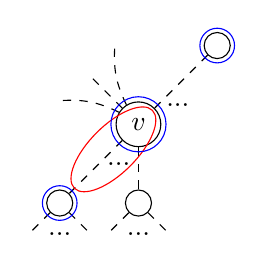
\begin{tikzpicture}
            \node[draw, circle] (a) at (1,1) {};
            \node[draw, circle] (b) at (0,0) {$v$};
            \node[draw, circle] (c) at (-1,-1) {};
            \node[draw, circle] (d) at (0,-1) {};
            \node at (-0.25,-0.5) {...};
            \node at (-1,-1.4) {...};
            \node at (0,-1.4) {...};
            \node at (0.5,0.25) {...};
    
            \draw[dashed] (a) -- (b); 
            \draw[dashed] (b) -- (c); 
            \draw[dashed] (b) -- (d); 
            \draw[dashed] (b) -- (-0.6,0.6); 
            \draw[dashed, bend left=15] (b) to (-0.3,1);
            \draw[dashed, bend right=15] (b) to (-1,0.3);
            \draw[dashed] (c) to (-1.4,-1.4);
            \draw[dashed] (c) to (-0.6,-1.4);
            \draw[dashed] (d) to (-0.4,-1.4);
            \draw[dashed] (d) to (0.4,-1.4);
    
            \draw[rotate=45, red] (-0.45, 0) ellipse (0.7 and 0.3); 
            \draw[blue] (a) circle (0.22);
            \draw[blue] (b) circle (.35);
            \draw[blue] (c) circle (.22);
    
        \end{tikzpicture}
        \caption*{A}
    \end{subfigure}
    \begin{subfigure}{.3\textwidth}
        \centering
        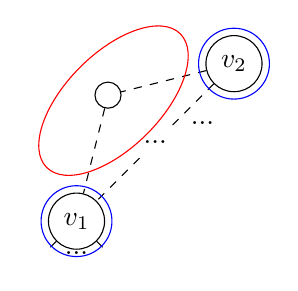
\begin{tikzpicture}
            \node[draw, circle] (a) at (1,1) {$v_2$};
            \node[draw, circle] (b) at (-0.6,0.6) {};
            \node[draw, circle] (c) at (-1,-1) {$v_1$};
    
            \node at (0.6,0.25) {...};
            \node at (0,0) {...};
            \node at (-1,-1.4) {...};
            
    
            \draw[dashed] (a) -- (b); 
            \draw[dashed] (b) -- (c); 
            \draw[dashed] (a) -- (0.2,0.2); 
            \draw[dashed] (-0.2,-0.2) -- (c); 
            
    
            \draw[dashed] (c) to (-1.4,-1.4);
            \draw[dashed] (c) to (-0.6,-1.4);
            
            \draw[rotate=45, red] (0, 0.75) ellipse (1.2 and 0.6); 
            \draw[blue] (a) circle (0.45);
            \draw[blue] (c) circle (.45);
            
        \end{tikzpicture}
        \caption*{B}
        \end{subfigure}
    \begin{subfigure}{.3\textwidth}
        \centering
        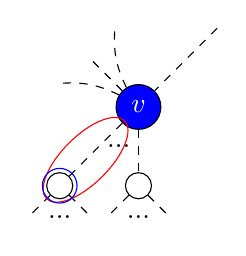
\begin{tikzpicture}
            \node[draw, circle, fill=blue] (b) at (0,0) {\textcolor{white}{$v$}};
            \node[draw, circle] (c) at (-1,-1) {};
            \node[draw, circle] (d) at (0,-1) {};
            \node at (-0.25,-0.5) {...};
            \node at (-1,-1.4) {...};
            \node at (0,-1.4) {...};
    
            \draw[dashed] (1,1) -- (b); 
            \draw[dashed] (b) -- (c); 
            \draw[dashed] (b) -- (d); 
            \draw[dashed] (b) -- (-0.6,0.6); 
            \draw[dashed, bend left=15] (b) to (-0.3,1);
            \draw[dashed, bend right=15] (b) to (-1,0.3);
            \draw[dashed] (c) to (-1.4,-1.4);
            \draw[dashed] (c) to (-0.6,-1.4);
            \draw[dashed] (d) to (-0.4,-1.4);
            \draw[dashed] (d) to (0.4,-1.4);
    
            \draw[rotate=45, red] (-0.95, 0) ellipse (0.7 and 0.3); 
            \draw[blue] (c) circle (.22);
    
        \end{tikzpicture}
        \caption*{C}
    \end{subfigure}
    \begin{subfigure}{.3\textwidth}
        \centering
        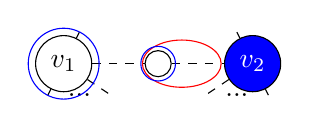
\begin{tikzpicture}
            \node[draw, circle] (a) at (-1.2,0) {$v_1$};			
            \node[draw, circle] (b) at (0,0) {};			
            \node[draw, circle, fill=blue] (c) at (1.2,0)  {\textcolor{white}{$v_2$}};
            
            \node at (-1,-0.4) {...};
            \node at (1,-0.4) {...};
    
            \draw[dashed] (a) -- (b);
            \draw[dashed] (b) -- (c);
            \draw[dashed] (a) -- (-1.4,-0.4);
            \draw[dashed] (a) -- (-0.6,-0.4);
            \draw[dashed] (a) -- (-1,0.4);
            
            \draw[dashed] (c) -- (1.4,-0.4);
            \draw[dashed] (c) -- (0.6,-0.4);
            \draw[dashed] (c) -- (1,0.4);
    
            \draw[red] (0.3, 0) ellipse (0.5 and 0.3); 
            \draw[blue] (a) circle (.45);
            \draw[blue] (b) circle (.22);
    
        \end{tikzpicture}
        \caption*{D}
    \end{subfigure}
    \begin{subfigure}{.3\textwidth}
        \centering
        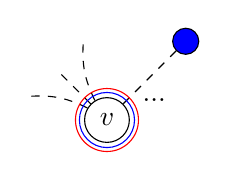
\begin{tikzpicture}
            \node[draw, circle, fill=blue] (a) at (1,1) {};
            \node[draw, circle] (b) at (0,0) {$v$};
            
            \node at (0.6,0.25) {...};
    
    
            \draw[dashed] (a) -- (b); 
            \draw[dashed] (b) -- (-0.6,0.6); 
            \draw[dashed, bend left=15] (b) to (-0.3,1);
            \draw[dashed, bend right=15] (b) to (-1,0.3);
            
            \draw[blue] (b) circle (.35);
            \draw[red] (b) circle (.4);
        \end{tikzpicture}        
        \caption*{E}
    \end{subfigure}
    \begin{subfigure}{.3\textwidth}
        \centering
        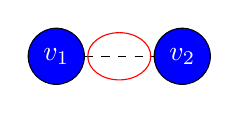
\begin{tikzpicture}
            \node[draw, circle, fill=blue] (a) at (-0.8,0) {\textcolor{white}{$v_1$}};
            \node[draw, circle, fill=blue] (b) at (0.8,0) {\textcolor{white}{$v_2$}};
        
            \draw[dashed] (a) -- (b);
            \draw[red] (0, 0) ellipse (0.4 and 0.3); 
        \end{tikzpicture}
        \vspace{1cm}
        \caption*{F}
    \end{subfigure}
    \begin{subfigure}{.3\textwidth}
    \end{subfigure}
    \begin{subfigure}{.3\textwidth}
    \end{subfigure}

    \caption{The red region shows the hiding spot of the robber. The blue circles are the cop-positions after the round. The blue verteces are places where the cops were placed in the last round and stay. Each dashed line represents a path of length $s$.}
    \label{fig:CopStragyTree}
\end{figure}


\TheoremVisLazyCopmonotonicity*
\begin{proof}
    For $s=1$, we can again use the graphs $G_n$ from the last proof, as all mentioned robber strategies already are lazy. For speeds $s>1$, we remove the back\-/vertices and instead add fresh paths of length $s+1$ to connect each core\-/vertex to each of its predecessors. The robber strategy against $n-1$ cop\-/monotone cops stays the same: He starts at the root and, first, lazily descendents down the tree, taking steps of size one. Second, when he reaches a leaf and a cop is moved on his position, there is an unguarded path of length $s+1$ towards one of its predecessors. He goes into that path the maximum distance of $s$ units and is safe at the predecessor in the next round. \\
    The cop strategy is similar as well: The robber is forced down the tree by placing a cop on the parent vertex and, in the next round, placing one on the robber's position. When the robber leaves the tree, he is at a vertex of degree two and can be caught by moving in the neighbourhood of his position and, in the next round, on the vertex itself. This works with three non\-/cop\-/monotone cops or $n$ cop\-/monotone ones.
\end{proof}

\TheoremLazyRecontamination*
\begin{proof}
    We prove that the graph $G$ in \cref*{fig:LazyRecontamination} has the claimed properties of $\vlcopwidth{4}(G)\leq\ilcopwidth{4}(G)\leq10$ and $\rmilcopwidth{4}(G)\geq\rmvlcopwidth{4}(G)>10$, which implies the theorem. $G$ contains two 8\=/cliques $A$ and $B$ and a 2\=/clique $C$. The other circles represent single vertices, while the vertex $v$ plays the central role outlined in the main text.
    Edges between one of the cliques and another vertex are meant as multiple edges, connecting each vertex of the clique with that vertex. 
    For both directions it suffices to prove the stronger case.
    \subsubsection{$\rmilcopwidth{4}(G)\geq\rmvlcopwidth{4}(G)>10$}
    A visible lazy robber with speed four can force ten cops to allow recontamination. He does that by staying in $A$ until it gets completely occupied by cops. Then, if $v$ is not guarded, he can move to $B$, since the remaining two cops could not block all connecting paths of length $\leq 4$ and repeat symmetrically. Otherwise, he can escape to $C$, as there are four paths of length four connecting $C$ to $A$ and $B$ and only one cop left. \\
Next either the robber moves to $A$ or $B$ and we are were we started or the cops need to position on $C$ and all eight paths of length $\leq 4$ that connect $C$ to either $A$ or $B$. However, when they do that no cops are left and he can move on $v$ breaking the robber\-/monotonicity.

    \subsubsection{$\vlcopwidth{4}(G)\leq\ilcopwidth{4}(G)\leq10$}
    We present a strategy for ten cops on the mentioned graph, by showing the positions of the cops (blue) and remaining hiding spots of the invisible robber (red) at each round $t$.
    \begin{longtable}{cc}
        \farbigergraph{red!60,red!60,red!60,red!60,red!60,red!60,red!60,red!60,red!60,red!60,red!60,red!60,red!60,red!60,red!60,red!60,red!60,red!60,red!60,red!60,red!60,red!60,red!60,red!60,red!60,red!60,red!60,red!60,red!60,red!60,red!60,red!60,red!60,red!60,red!60,red!60,red!60,red!60} &  \farbigergraph{blue,red!60,red!60,red!60,red!60,red!60,blue,red!60,red!60,red!60,red!60,red!60,red!60,red!60,red!60,red!60,red!60,red!60,red!60,red!60,red!60,red!60,red!60,red!60,red!60,red!60,red!60,red!60,red!60,red!60,red!60,red!60,red!60,red!60,red!60,red!60,blue} \\
        t=0 & t=1 \\
        \farbigergraph{blue,red!60,red!60,red!60,red!60,red!60,white,blue,red!60,red!60,red!60,red!60,red!60,red!60,red!60,red!60,red!60,red!60,red!60,red!60,red!60,red!60,red!60,red!60,red!60,red!60,red!60,red!60,red!60,red!60,red!60,red!60,red!60,red!60,red!60,red!60,blue} &  \farbigergraph{blue,red!60,red!60,red!60,red!60,red!60,white,white,blue,red!60,red!60,red!60,red!60,red!60,red!60,red!60,red!60,red!60,red!60,red!60,red!60,red!60,red!60,red!60,red!60,red!60,red!60,red!60,red!60,red!60,red!60,red!60,red!60,red!60,red!60,red!60,blue} \\
        t=2 & t=3 \\
        \farbigergraph{blue,red!60,red!60,red!60,red!60,red!60,white,white,white,red!60,red!60,red!60,blue,red!60,red!60,blue,red!60,red!60,red!60,red!60,red!60,red!60,red!60,red!60,red!60,red!60,red!60,red!60,red!60,red!60,red!60,red!60,red!60,red!60,red!60,red!60,white} &  \farbigergraph{blue,red!60,red!60,red!60,red!60,red!60,white,white,white,red!60,red!60,red!60,white,red!60,red!60,white,red!60,red!60,blue,red!60,red!60,blue,red!60,red!60,red!60,red!60,red!60,red!60,red!60,red!60,red!60,red!60,red!60,red!60,red!60,red!60,white} \\
        t=4 & t=5 \\
        \farbigergraph{white,blue,red!60,blue,red!60,red!60,white,white,white,red!60,red!60,red!60,white,red!60,red!60,white,red!60,red!60,white,red!60,red!60,white,red!60,red!60,red!60,red!60,red!60,red!60,red!60,red!60,red!60,red!60,red!60,red!60,red!60,red!60,blue} &  \farbigergraph{white,blue,red!60,white,blue,red!60,white,white,white,red!60,red!60,red!60,white,red!60,red!60,white,red!60,red!60,white,red!60,red!60,white,red!60,red!60,red!60,red!60,red!60,red!60,red!60,red!60,red!60,red!60,red!60,red!60,red!60,red!60,blue} \\
        t=6 & t=7 \\
        \farbigergraph{white,blue,red!60,white,white,blue,white,white,white,red!60,red!60,red!60,white,red!60,red!60,white,red!60,red!60,white,red!60,red!60,white,red!60,red!60,red!60,red!60,red!60,red!60,red!60,red!60,red!60,red!60,red!60,red!60,red!60,red!60,blue} &  \farbigergraph{white,blue,red!60,white,white,white,white,white,white,red!60,red!60,red!60,white,red!60,red!60,white,red!60,red!60,white,red!60,red!60,white,red!60,red!60,blue,red!60,red!60,blue,red!60,red!60,red!60,red!60,red!60,red!60,red!60,red!60,white} \\
        t=8 & t=9 \\
        \farbigergraph{white,blue,red!60,white,white,white,white,white,white,red!60,red!60,red!60,white,red!60,red!60,white,red!60,red!60,white,red!60,red!60,white,red!60,red!60,white,red!60,red!60,white,red!60,red!60,blue,red!60,red!60,blue,red!60,red!60,white} &  \farbigergraph{white,white,red!60,white,white,white,white,white,white,red!60,red!60,red!60,blue,red!60,red!60,blue,red!60,red!60,blue,red!60,red!60,blue,red!60,red!60,blue,red!60,red!60,blue,red!60,red!60,blue,red!60,red!60,blue,red!60,red!60,white} \\
        t=10 & t=11 \\
        \farbigergraph{white,white,red!60,white,white,white,white,white,white,red!60,red!60,red!60,blue,red!60,red!60,blue,red!60,red!60,blue,red!60,red!60,blue,red!60,red!60,blue,red!60,red!60,blue,red!60,red!60,blue,blue,red!60,blue,blue,red!60,white} &  \farbigergraph{white,white,red!60,white,white,white,white,white,white,red!60,red!60,red!60,blue,red!60,red!60,blue,red!60,red!60,blue,red!60,red!60,blue,red!60,red!60,blue,blue,red!60,blue,blue,red!60,white,blue,red!60,white,blue,red!60,white} \\
        t=12 & t=13 \\
        \farbigergraph{white,white,red!60,white,white,white,white,white,white,red!60,red!60,red!60,blue,red!60,red!60,blue,red!60,red!60,blue,red!60,red!60,blue,red!60,red!60,white,blue,red!60,white,blue,red!60,white,blue,blue,white,blue,blue,white} &  \farbigergraph{white,white,red!60,white,white,white,white,white,white,red!60,red!60,red!60,blue,red!60,red!60,blue,red!60,red!60,blue,red!60,red!60,blue,red!60,red!60,white,blue,blue,white,blue,blue,white,white,blue,white,white,blue,white} \\
        t=14 & t=15 \\
        \farbigergraph{white,white,red!60,white,white,white,white,white,white,red!60,red!60,red!60,blue,blue,red!60,blue,blue,red!60,blue,red!60,red!60,blue,red!60,red!60,white,white,blue,white,white,blue,white,white,blue,white,white,blue,white} &  \farbigergraph{white,white,red!60,white,white,white,white,white,white,red!60,red!60,red!60,white,blue,red!60,white,blue,red!60,blue,blue,red!60,blue,blue,red!60,white,white,blue,white,white,blue,white,white,blue,white,white,blue,white} \\
        t=16 & t=17 \\
        \farbigergraph{white,white,red!60,white,white,white,white,white,white,red!60,red!60,red!60,white,blue,blue,white,blue,blue,white,blue,red!60,white,blue,red!60,white,white,blue,white,white,blue,white,white,blue,white,white,blue,white} &  \farbigergraph{white,white,red!60,white,white,white,white,white,white,red!60,red!60,red!60,white,white,blue,white,white,blue,white,blue,blue,white,blue,blue,white,white,blue,white,white,blue,white,white,blue,white,white,blue,white} \\
        t=18 & t=19 \\
        \farbigergraph{white,white,blue,white,white,white,white,white,white,red!60,red!60,red!60,white,white,blue,white,white,blue,white,white,blue,white,white,blue,white,white,blue,white,white,blue,white,white,blue,white,white,blue,red!60} &  \farbigergraph{white,white,blue,blue,blue,blue,blue,blue,blue,red!60,red!60,red!60,white,white,white,white,white,white,white,white,white,white,white,white,white,white,white,white,white,white,white,white,white,white,white,white,red!60} \\
        t=20 $\rightarrow$ Recontamination! & t=21 \\
        \farbigergraph{white,white,blue,blue,blue,blue,blue,blue,blue,red!60,red!60,red!60,white,white,white,white,white,white,white,white,white,white,white,white,white,white,white,white,white,white,white,white,white,white,white,white,blue} &  \farbigergraph{white,white,blue,white,white,white,white,white,white,blue,blue,blue,white,white,white,white,white,white,white,white,white,white,white,white,white,white,white,white,white,white,white,white,white,white,white,white,blue} \\
        t=22 & t=23 $\rightarrow$ Cleared! \\
    
    \end{longtable}
    For higher speeds $s\geq4$, one can adjust $G$ by replacing the paths of length four between $C$ and $A$, $C$ and $B$, and $C$ and $v$ by paths of length $s$. The strategies for the cops or, respectively, the robber trivially generalise.
\end{proof}

\LemmaVisLazyFunnelToStrat*
\begin{proof}
    We give a strategy for $k+1$ cops: If the robber is on vertex $v$ then move cops on $cut(F(v))$ or if they are already positioned there move an extra cop on $v$.
    Formally, choose $$S_{i+1} = \begin{cases}
        cut(F(R_i)) \cup \{R_i\},  & \text{if } S_i = cut(F(R_i)) \\
        cut(F(R_i)),  &  \text{otherwise.}
    \end{cases}$$
    The robber will be forced to move at least every second round and by definition of the cut, every path form $F(R_i)$ to $V\setminus F(R_i)$ will be blocked by a cop in this round. It follows that $F(R_0)\supsetneq F(R_2) \supsetneq ... F(R_{2k})$ for every $k$ until $F(R_{2k}) = \{R_{2k}\}$ and the robber gets caught.
    This strategy uses $k+1$ cops. Now for the cop monotonicity we want to prove for $i<j<k$: $$S_i\cap S_k \subseteq S_j.$$
    For $v\in S_i\cap S_k$ we have that
    \begin{align*}
        v\in S_i &\implies v=R_{i-1} \vee v\in cut(F(R_{i-1})) \\
        &\implies v\notin F(R_i) \ \ \ (*) \\
        &\implies v\notin F(R_{j-1})
    \end{align*}
    we also have 
    \begin{align*}
        v\in S_k &\implies v=R_{k-1} \vee v\in cut(F_{k-1})\\
        &\overset{by (*)}{\implies} v\in cut(F(R_{k-1})) \\
        &\implies \exists u\in F(R_{k-1}): \ (v,u)\in E \\ 
        &\implies \exists u\in F(R_{j-1}): \ (v,u)\in E \\ 
    \end{align*}
    Put together we have $v\in cut(F_{j-1}) \subseteq S_j$, so the strategy induced by our monotone funnel is cop\-/monotone.
\end{proof}

\LemmaVisLazyStratToFunnel*
\begin{proof}
    We use induction over $j \leq |V|$ to prove our claim that there exists an $A_j\subseteq V$ with $|A_j|=j$ and a monotone funnel $F_j$ on $A_j$ of width less then $k$. The theorem then follows from the case $j=|V|$. Note that our proof is not constructive, even though an optimal funnel can indeed be constructed efficiently. \\
    \underline{Basecase:} For $j=0$ use $A_0=\emptyset$ and $F_j$ the empty function.\\
    \underline{Inudctive Case:} Assume the inductive hypthesis, so the existence of proper $A_j$ and $F_j$ for some $j<|V|$. Of the possible monotone funnels on $A_j$, like $F_j$, choose $F$ to be minimal in the sense, that for every other monotone funnel $F'$ on $A_j$ of width less then $k$ and $F'(a)\subseteq F(a)$ for all $a\in A_j$ we have $F=F'$. We want to work with this minimal $F$ because for the corresponding cop\-/strategy it means, that the options for the robber to move should be inclusionwise minimal. \\
    Now since $V\setminus A_j$ is not a $(k,\infty)$\=/hideout (see appendix or \cite{doi:10.1137/090780006} for definition) there is a $x\in V \setminus A_j$ and a $C\subseteq V \setminus \{x\}$ with $|C| < k$ such that $G\setminus C$ does not contain a path from $x$ to $V\setminus A$. So with this $C$ there is an extension of $F$ to the domain $A_{j+1} = A \cup \{x\}$ by setting $F(x)$ to the connected component of $x$ in $G\setminus C$ and this is a funnel of width less then $k$. For $x$ $\mathit{(F1,F3)}$ are trivial and $\mathit{(F2)}$ follows from the fact that $x\notin A_j$.
    For reasons that become clear later we choose from the possibilities of such extension of $F$ (we showed above that there is at least one) the one funnel $F_{j+1}$ that is inclusionwise maximal in regards to $F(x)$. \\
    Lets take a step back and look at what we have: A funnel $F_{j+1}$ on $A_{j+1}$ such that $F_{j+1}(x)$ is maximal, $F_{j+1}(a)$ is minimal for $a\in A_j$ and $F_{j+1}$ is already monotone on $A_j$. We claim that it is monotone on whole $A_{j+1}$:\\
    For contradiction assume that this is not the case, then there is a $y\in F_{j+1}(x)$ such that $F_{j+1}(y)\not\subseteq F_{j+1}(x)$. Let $y$ be minimal in regards to $F_{j+1}$ with that property, meaning that for $y'\in F_{j+1}(x)\cap F_{j+1}(y)$ $F_{j+1}(y')\subseteq F_{j+1}(x)$. Then let $Z$ denote the area of non\-/monotonicity $F_{j+1}(y)\cap cut(F_{j+1}(x))$ which is not empty. Corresponding to our strategy we could say that from $x$ the cops allow the robber to move to $y$ and guard the vertices $Z$ that are next to $y$, while from $y$ they then allow him the freedom to move on $Z$ but therefore have to guard some other region $\hat{Z}$. We denote this area $\hat{Z} := cut(F_{j+1}(x) \cup F_{j+1}(y)) \setminus cut(F_{j+1}(x))$.\\ 
    To get a better picture these relations are depicted in \cref{fig:VisLazyDipiction}. Our definitions of $Z$ and $\hat{Z}$ are fruitful, because they satisfy the following equations (calculations can be found further down):
    \begin{equation}
        cut(F_{j+1}(x) \cup F_{j+1}(y))=(cut(F_{j+1}(x))\setminus Z) \cup \hat{Z}\\
        \label{Calc1}
    \end{equation}
    \begin{equation}
        cut(F_{j+1}(x) \cap F_{j+1}(y))\subseteq (cut(F_{j+1}(y))\setminus \hat{Z}) \cup Z
        \label{Calc2}
    \end{equation}
    \begin{equation}
        \hat{Z} \subseteq cut(F_{j+1}(y))
        \label{Calc3}
    \end{equation}
    
    \begin{figure}
    \centering
    \begin{tikzpicture}
        \pgfdeclarelayer{background}
        \pgfdeclarelayer{main}
        \pgfsetlayers{background,main}

        \node[draw, circle] (x) at (0,0) {$x$};
        \node[draw, circle, fill=blue!75] (A) at (-1,0) {};
        \node[draw, circle, shading=splitshading] (B) at (1,1) {};
        \node[draw, circle, fill=orange!50] (M) at (1,0) {};
        \node[draw, circle] (Y) at (2,0) {$y$};
        \node[draw, circle, shading=splitshading] (C) at (1,-1) {};
        \node[draw, circle, fill=blue!75] (Z1) at (3,1) {};
        \node[draw, circle, fill=blue!75] (Z2) at (3,0) {};
        \node[draw, circle, fill=blue!75] (Z3) at (3,-1) {};
        \node[draw, circle] (F) at (4,-0.5) {};
        \node[draw, circle, fill=orange!50] (ZH1) at (5,0.33) {};
        \node[draw, circle, fill=orange!50] (ZH2) at (5,-0.33) {};
        \node[draw, circle] (D) at (6,1) {};
        \node[draw, circle] (E) at (6,0) {};

        \draw (A) -- (x)
                (x) -- (M)
                (B) -- (M)
                (B) -- (Z1)
                (M) -- (Y)
                (Y) -- (C)
                (Z1) -- (Y)
                (Z2) -- (Y)
                (Z3) -- (Y)
                (Z3) -- (F)
                (Z1) -- (ZH1)
                (Z2) -- (ZH1)
                (F) -- (ZH1)
                (F) -- (ZH2)
                (ZH1) -- (D)
                (ZH1) -- (E);
    \begin{pgfonlayer}{background}
        \node[draw, dashed, fit=(ZH1) (ZH2), inner sep=5pt, label=above:{\(\hat{Z}\)}] {};

        \node[draw, dashed, fit=(Z1) (Z2) (Z3), inner sep=8pt, label=above:{\(Z\)}] {};

        \node[draw=blue,rounded corners, fill=blue!35, fill opacity=0.5, fit=(x) (M) (Y), inner sep=5pt, label=below left:{\(F_{j+1}(x)\)}] {};

        \node[draw=orange,rounded corners, fill=orange!20, fill opacity=0.5, fit=(Y) (Z1) (Z2) (Z3) (F), inner sep=5pt,label=below right:{\(F_{j+1}(y)\)}] {};
    \end{pgfonlayer}
    \end{tikzpicture}

    \caption{Depiction of the different elements in the proof of \cref{thmt@@LemmaVisLazyStratToFunnel}. The dashed boxes represent the sets \(\hat{Z}\) and \(Z\), the light blue box represents the set \(F_{j+1}(x)\), and the orange box represents the set \(F_{j+1}(y)\). The blue and orange colored vertices are the vertices in the sets \(cut(F_{j+1}(x))\) and \(cut(F_{j+1}(y))\), respectively.}
    \label{fig:VisLazyDipiction}
\end{figure}


    With all of this build up we can make a case distinction on the sizes of $Z$ and $\hat{Z}$ and derive contradictions in both cases.\\
    \subsubsection{Case $|\hat{Z}| \leq |Z|$:}
    We have that $$\hat{F}: A_{j+1} \rightarrow \mathcal{P}ot(A_{j+1}), v \mapsto \begin{cases}
        F_{j+1}(v) & \text{if } v \in A_j\\
        F_{j+1}(x) \cup F_{j+1}(y) & \text{if } v=x
    \end{cases}$$
    is also a funnel. Its width is less then $k$ since 
    
    \begin{align*}
        |cut(\hat{F}(x))| &\overset{\cref*{Calc1}}{=} |\left(cut(F_{j+1}(x))\setminus Z \right) \cup \hat{Z}|\\
        &= |cut(F_{j+1}(x))| - |Z| + |\hat{Z}|\\
        &\leq |cut(F_{j+1}(x))|\\
        &< k,
    \end{align*}
    
    but $\hat{F}(x)\supsetneq F_{j+1}(x)$ which contradicts that $F_{j+1}(x)$ was maximal.\\

    \subsubsection{Case $|\hat{Z}| > |Z|$:}
    We have that $$\hat{F}: A \rightarrow \mathcal{P}ot(A), a \mapsto \begin{cases}
        F_{j+1}(a) & \text{if } a \neq y\\
        F_{j+1}(x) \cap F_{j}(y) & \text{if } a=y
    \end{cases}$$
    is also a target funnel. Its width is less then $k$ since 

    \begin{align*}
        |cut(\hat{F}(y))| &\overset{\cref*{Calc2}}{\leq} |\left(cut(F_{j+1}(y))\setminus \hat{Z}\right) \cup Z|\\
        &\leq |cut(F_{j+1}(y)) \setminus \hat{Z}| + |Z|\\
        &\overset{\cref*{Calc3}}{=} |cut(F_{j+1}(y))| - |\hat{Z}| + |Z|\\
        &< |cut(F_{j+1}(y))|\\
        &< k
    \end{align*}

    and it is moreover monotone since 
    $$\forall a \in A \setminus \{y\} \forall b \in \hat{F}(a): \ \hat{F}(b) \subseteq F_{j+1}(b) \subseteq F_{j+1}(a) = \hat{F}(a)$$
    
    and for all $b\in \hat{F}(y)=F_{j+1}(x)\cap F_{j+1}(y)$ the minimality of $y$ implies $\hat{F}(b) \subseteq F_{j+1}(x)$ and the monotonicity of $F$ implies $\hat{F}(b) \subseteq F_{j+1}(y)$. Thus $\hat{F}(b) \subseteq F_{j+1}(x)\cap F_{j+1}(y)=\hat{F}(y)$. But $\hat{F}(y)\subsetneq F_{j+1}(y)$ which contradicts that $F_{j+1}$ and therefore $F$ was minimal on $A_j$. \\

    So overall $F_{j+1}$ has to be monotone on $A_{j+1}$ and we have proven the inductive step. The only thing left are the three equations from earlier:\\
\underline{Claim $cut(F_{j+1}(x) \cup F_{j+1}(y))=(cut(F_{j+1}(x))\setminus Z) \cup \hat{Z}$:}\\
\begin{align*}
    \left(cut(F_{j+1}(x))\setminus Z\right) \cup \hat{Z} =&\ \left(cut(F_{j+1}(x))\setminus F_{j+1}(y)\right) \cup \hat{Z} \\
    =&\ \left\{v \in  V\setminus \left( F_{j+1}(x)\cup F_{j+1}(y)\right) \ | \ \exists t \in F_{j+1}(x): \ (t,v)\in E  \right\} \cup \hat{Z} \\
    =&\ \left(cut\left(F_{j+1}(x) \cup F_{j+1}(y)\right) \cap cut\left(F_{j+1}(x)\right)\right) \\
    & \cup (cut(F_{j+1}(x) \cup F_{j+1}(y)) \setminus cut(F_{j+1}(x)))\\
    =&\ cut(F_{j+1}(x) \cup F_{j+1}(y))
\end{align*}
\underline{Claim $cut(F_{j+1}(x) \cap F_{j+1}(y))\subseteq (cut(F_{j+1}(y))\setminus \hat{Z}) \cup Z$:}\\
\begin{align*}
    (cut(F_{j+1}(y))\setminus \hat{Z}) \cup Z =& \left(cut(F_{j+1}(y))\setminus cut(F_{j+1}(x) \cup F_{j+1}(y))\right) \\
    &\cup \left(cut(F_{j+1}(y)) \cap cut(F_{j+1}(x))\right) \\
    &\cup Z \\
    =& \{v \in F_{j+1}(x)\setminus F_{j+1}(y) \ | \ \exists t \in F_{j+1}(y): \ (t,v)\in E\} \\
    &\cup \{v \in V\setminus (F_{j+1}(y) \cup F_{j+1}(x)) \ | \ \exists t \in F_{j+1}(y): \ (t,v)\in E \\
    &\hspace{5cm}                                        \wedge \exists t \in F_{j+1}(x): \ (t,v)\in E\}\\
    &\cup \{v \in F_{j+1}(y)\setminus F_{j+1}(x) \ | \ \exists t \in F_{j+1}(x): \ (t,v)\in E\} \\
    \supseteq& \{v \in F_{j+1}(x)\setminus F_{j+1}(y) \ | \ \exists t \in F_{j+1}(x)\cap F_{j+1}(y): \ (t,v)\in E\}\\
    &\cup \{v \in V\setminus (F_{j+1}(y) \cup F_{j+1}(x)) \ | \ \exists t \in F_{j+1}(x) \cap F_{j+1}(y): \ (t,v)\in E \}\\
    &\cup \{v \in F_{j+1}(y)\setminus F_{j+1}(x) \ | \ \exists t \in F_{j+1}(x) \cap F_{j+1}(y): \ (t,v)\in E\}\\
    =& cut(F_{j+1}(x) \cap F_{j+1}(y))
\end{align*}
\underline{Claim $\hat{Z} \subseteq cut(F_{j+1}(y))$}
\begin{align*}
    \hat{Z} =& cut(F_{j+1}(x) \cup F_{j+1}(y)) \setminus cut(F_{j+1}(x))\\
    \subseteq& \{v \in V\setminus \left(F_{j+1}(x) \cup F_{j+1}(y)\right) \ | \ \exists t \in \left(F_{j+1}(x) \cup F_{j+1}(y)\right): \ (t,v)\in E\} \\
    &\setminus \{v \in V\setminus \left(F_{j+1}(x) \cup F_{j+1}(y)\right) \ | \ \exists t \in F_{j+1}(x): \ (t,v)\in E\}\\
    \subseteq& \{v \in V\setminus F_{j+1}(y) \ | \ \exists t \in F_{j+1}(y): \ (t,v)\in E\} \\
    =& cut(F_{j+1}(y))
\end{align*}
\qed
\end{proof}